\documentclass[border=2pt]{standalone}
\usepackage{pgfplots}
\usepackage{pgfplotstable}
\pgfplotsset{compat=1.18}
\usepackage{xcolor}
\definecolor{amber}{HTML}{E69F00}
\definecolor{teal}{HTML}{009E73}
\definecolor{blue}{HTML}{0072B2}
\definecolor{mauve}{HTML}{CC79A7}
\definecolor{grey}{HTML}{999999}
\definecolor{vermilion}{HTML}{D55E00}
\usepackage{times}

\begin{document}

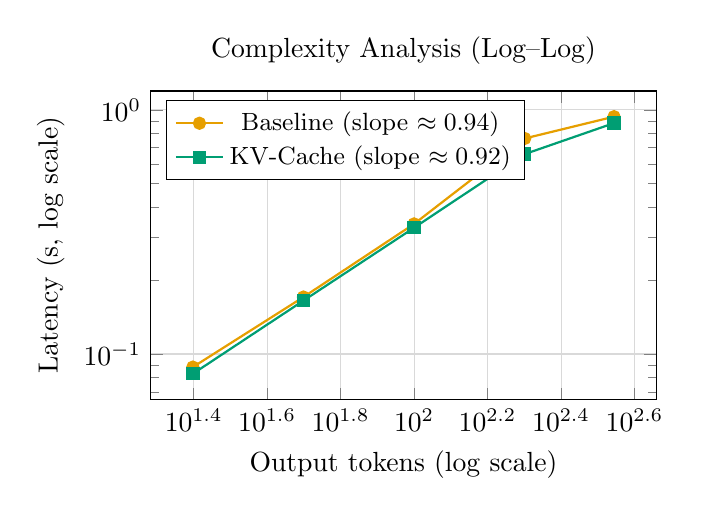
\begin{tikzpicture}
\begin{axis}[
  width=8cm, height=5.5cm,
  xmode=log, ymode=log,
  xlabel={Output tokens (log scale)},
  ylabel={Latency (s, log scale)},
  title={Complexity Analysis (Log--Log)},
  legend pos=north west,
  legend style={font=\small},
  grid=major, grid style={gray!30},
]
\addplot[color=amber, mark=*, thick] coordinates {(25,0.0884) (50,0.1712) (100,0.3412) (200,0.7639) (350,0.9382)};
\addlegendentry{Baseline (slope $\approx 0.94$)}
\addplot[color=teal, mark=square*, thick] coordinates {(25,0.0830) (50,0.1655) (100,0.3292) (200,0.6591) (350,0.8829)};
\addlegendentry{KV-Cache (slope $\approx 0.92$)}
\end{axis}
\end{tikzpicture}
\end{document}
